\documentclass{article} % For LaTeX2e
\usepackage{graphicx}
\graphicspath{ {images/} }
\usepackage{nips14submit_e,times}
\usepackage{hyperref}
\usepackage{cleveref}
\usepackage{subcaption}
\usepackage{url}
%\documentstyle[nips14submit_09,times,art10]{article} % For LaTeX 2.09

\title{Automatic Target Detection and Classification: \\
  Deep Learning on Low Power Platforms}

\author{
  Asst. Prof. Mark Silberstein \\
  mark@ee.technion.ac.il\\
}

\newcommand{\fix}{\marginpar{FIX}}
\newcommand{\new}{\marginpar{NEW}}

\nipsfinalcopy % Uncomment for camera-ready version

\newcommand{\cropsrow}[3]{\includegraphics[width=0.15\textwidth]{images/crops/#1.jpg} & #2 & \includegraphics[width=0.15\textwidth]{images/crops/mask_#1.jpg} & #3}

\begin{document}

\maketitle

\section{Summary}

Over the last decades the use of Unmanned System (US) has proved very beneficial in
saving life of military personal and cutting the costs of operational tasks.
However, these systems still require a `Man in the loop' for remote control, scene
recognition, and data acquisition, 
thereby increasing the cost of operation and significantly limiting the scope of 
applications to those in which such a remote control is possible.

On the other hand, recent years have seen revolutionary advancements in machine learning
algorithms. The new class of algorithms, called Deep Neural Networks (DNN), have
been shown to enable 
computers accomplish image classification and recognition tasks previously
considered tractable only by humans. The tremendous potential of these
algorithms in solving recognition tasks in Unmanned Systems is apparent, as 
their use may bring real-time human-level vision capabilities and pave the way
toward fully Unmanned Autonomous Systems (UAS).
Unfortunately, the typically scarce computing capacity of unmanned systems,
primarily due to strict weight and size constraints, make the application of the
existing compute-greedy deep neural network-based algorithms extremely challenging. 

This proposal aims to bring the power of deep neural networks to Unmanned
Systems via three main research thrusts:

\begin{itemize}
	\item Optimization of the structure of deep neural networks for specific
		recognition tasks encountered in (US), like object recognition,
		TODO: ADD MORE 
\item The design and implementation of the algorithms focusing on power
	efficiency, by leveraging a new  class of high
	performance low-power commodity platforms with embedded Graphics
	Processing Units, like  NVIDIA Jetson TX1.
\item  TODO: Something else???
\end{itemize}

TODO: AMIT - explain in 2 sentences how you can optimize the structure of a DNN.

Graphics Processing Units are now routinely used as high-performance
accelerators in Supercomputing workloads, and in particular, for training deep neural
network.  In this proposal we seek to take advantage of a novel hybrid CPU-GPU architecture 
of embedded GPUs to leverage their computing capacity for low-power
\emph{inference} tasks. Combined with the new generation of low power embedded
systems like NVIDIA Jetson TX1,  our optimized power-optimized inference holds
the potential to empower complex classification and recognition tasks on the
Unmanned System. 

Critically, throughout the intermediate steps of this project as well as its
final results will be evaluated on a real Unmanned Aerial Vehicle (UAV), in cooperation with the Technion AUVSI project
team which is a collaboration between the Aerospace and Electrical engineering
faculties. 
%in which students design and build Unmanned Autonomous aerial system
%to compete in the AUVSI students competition.




\section{Background}

\subsection{Deep Learning}
\label{sec:deep_learning}

Classical machine learning, traditionally approaches classification problems
by first transforming the data from the problem space to some feature
space. The data in this feature space is hopefully invariant to transforms common
in the problem space, e.g. similarity and affine transforms, occlusion, lighting
etc. It is assumed that in this feature space, objects of the same class reside
in some manifold and the manifolds of different objects are separated by regions
of low density. A classifier, e.g. SVM is trained on this feature space to
discriminate between object of different classes.

This approach has been applied successfully to problems in many fields. But
finding the right
feature space for the problem and the right classifier for the feature space is
a complicated task that requires expertise.

During the last years, Deep Learning (DL)~\cite{Bengio2009, LeCun2015} proved to be the De-facto method for
many artificial intelligence tasks. One of the main advantages of DL is that
it automatically learns the feature space. Thus the feature space is custom
tailored for the specific problem.

\subsection{General-purpose computing on graphics processing units}

General-purpose computing on graphics processing units is the use of a
graphics processing unit (GPU),to perform computation in applications traditionally
handled by the central processing unit (CPU). The advantage of a GPU over a
CPU comes from the fact that it is designed for Single Instruction Multiple Data (SIMD) tasks.
Therefore it is fit for numerical operations like matrix multiplication
which lie in the heart of Deep Learning frameworks. The GPU can usually speedup
the calculation of a DL network by an order of magnitude compared to a CPU.

\subsection{AUVSI project}

The Association for Unmanned Vehicle Systems International (AUVSI)
organizes the Student Unmanned Aerial System (SUAS) competition
\url{http://www.auvsi-seafarer.org/}. The competition is aimed  at
stimulating and fostering interest in unmanned system technologies.
The  student  are required  to  develop  and  provide  the  analysis,
design, fabrication and demonstration of a system capable of completing
specific autonomous aerial missions.

One of the missions is the automatic detection and classification of targets.
Some targets are characterized by different geometric shapes and color. Another
target, in the form of a QR code requires high spatial resolution. Another
target is a doll in the form and size of a human. This target simulates
a search and rescue operation.~\cref{fig:targets} shows
some of the targets used in last year's competition.
\begin{figure}[h]
	\centering
	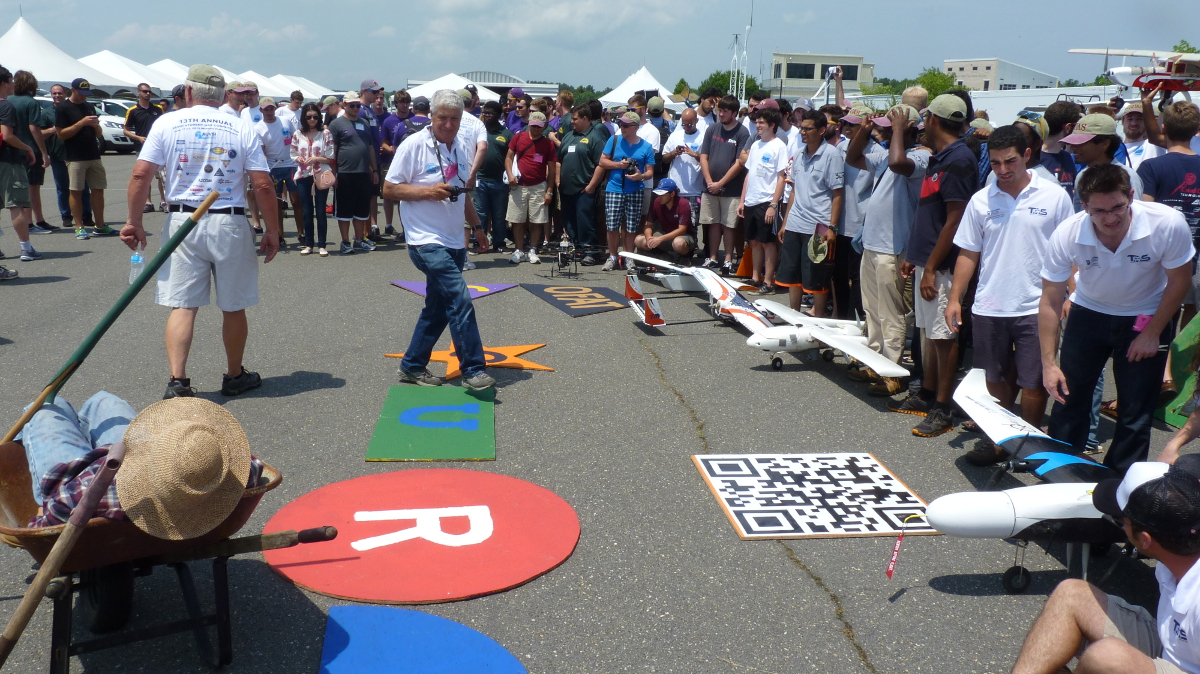
\includegraphics[width=0.8\textwidth]{auvsi_targets}
	\caption{Example of targets used in the 2015 AUVSI competition.}
	\label{fig:targets}
\end{figure}

This is the third year that the Technion participates in the AUVSI SUAS
competition. Last year the Technion team achieved 2\textsuperscript{nd} place
among more than 30 teams from universities all around the world.

\section{Proposed Research}

TODO: Amit, there should be a much better separation between the new ideas and
the preliminary results. Break it into two sections - just like I did in the
summary. 

For your subsection you basically should explain what you have already
done, as if you are still not sure if it will work, and explain how it is
different from the state of the art. And then you add "preliminary results" that
show that your initial idea was right, but there's still a lot to be done, e.g.,
improve the structure, remove layers, try other network architcetures, etc..

For the embedded GPU stuff - you can add a bunch of things that you can copy
from Ahmad's work, where again, try as much as you can to split between "future"
and now. Also I would add a subseciton which is called "evaluation and
integration with real systems" and then talk at length about AUVSI. 



\subsection{Target Detection and Classification}

The task of target detection and classification is related
to surveillance, `search and rescue', `friend or foe' identification and many other security related missions. 
The Region Convolutional Neural Networks
(R-CNN)~\cite{Girshick2014}, introduced in 2014 ,revolutionized the area of object detection, classification, and segmentation.
Fig.~\ref{fig:RCNN} show the diagram of a typical
R-CNN system. It is made of two stages, the first is a region proposal stage that extracts
object candidates. This regions are stretched into a predefined patch size and then
fed into a CNN. The CNN calculates confidence levels for a set of objects it was trained
for.
\begin{figure}[h]
	\centering
	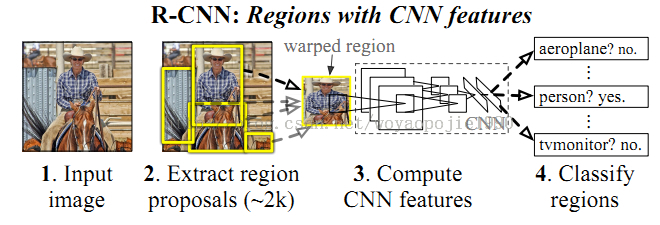
\includegraphics[width=0.8\textwidth]{RCNN}
	\caption{Diagram of a RCNN system}
	\label{fig:RCNN}
\end{figure}

We implemented a system based on R-CNN architecture to detect and classify the
targets in the AUVSI competition. The system is comprised of two subsystems shown
in~\cref{fig:shape_diagram,fig:letter_diagram}.
\begin{figure}[h]
	\centering
	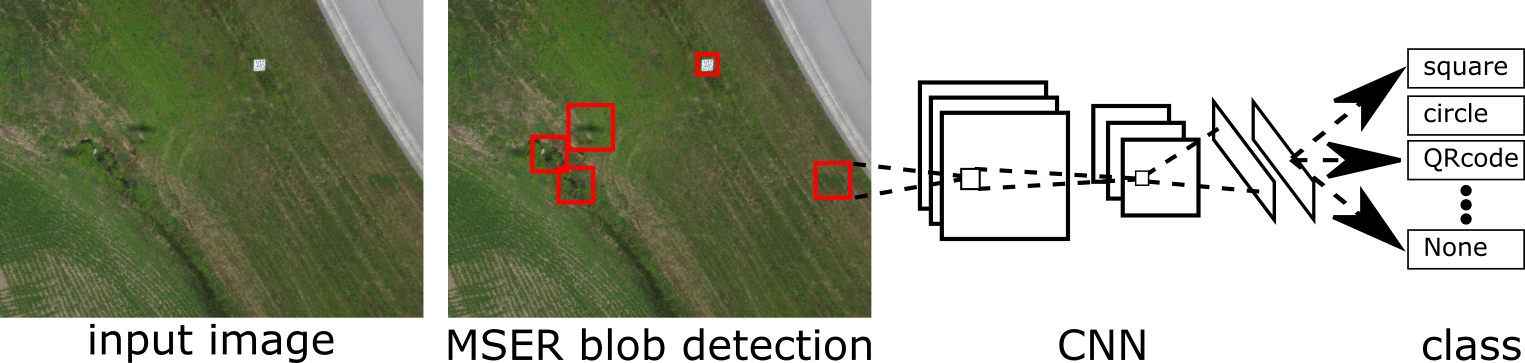
\includegraphics[width=0.8\textwidth]{diagram}
	\caption{Diagram of the shape classification subsystem}
	\label{fig:shape_diagram}
\end{figure}
\begin{figure}[h]
	\centering
	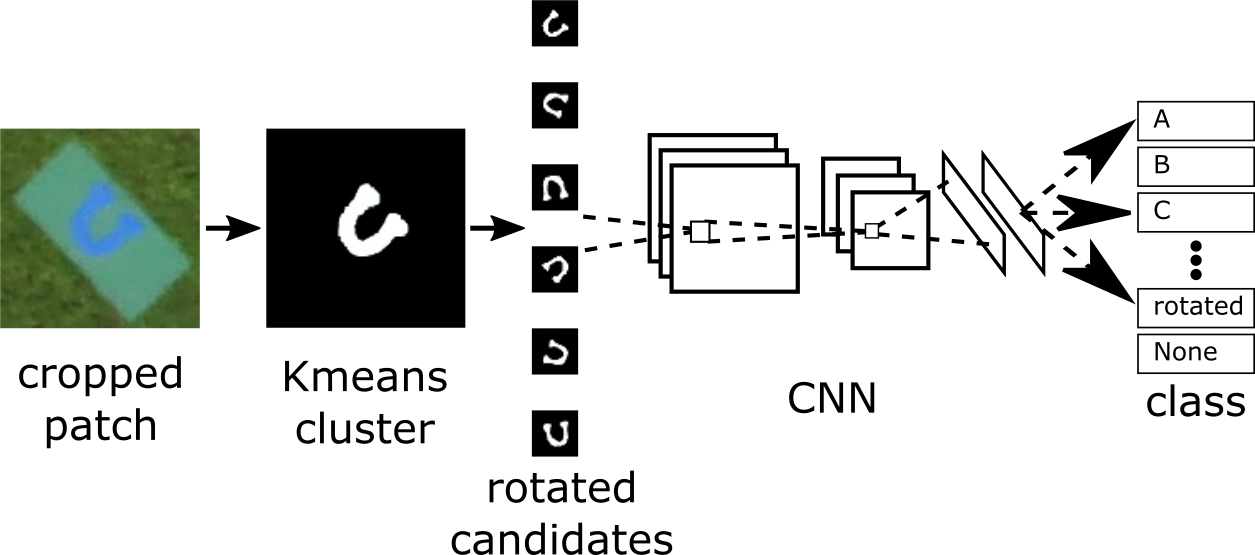
\includegraphics[width=0.5\textwidth]{letter_diagram}
	\caption{Diagram of the character classification subsystem}
	\label{fig:letter_diagram}
\end{figure}
The first subsystem detects and classifies target shapes in full (downscaled) image. The
input to this subsystem is a down-sampled version of the original image. The output
are square regions classified as one of the possible target shapes (circle, half circle,
cross, rectangle, etc.). These regions are croped from the full resolution
image and fed into the next subsystem that classifies the characters inside the shape. These subsystems
thus work as a cascade of classifiers. This hierarchical coarse to fine setup enables good
classification performance using smaller DL networks. \Cref{fig:true_positive2} shows an example of
an automatic detection and classification of a target.
\begin{figure}[h]
	\centering
	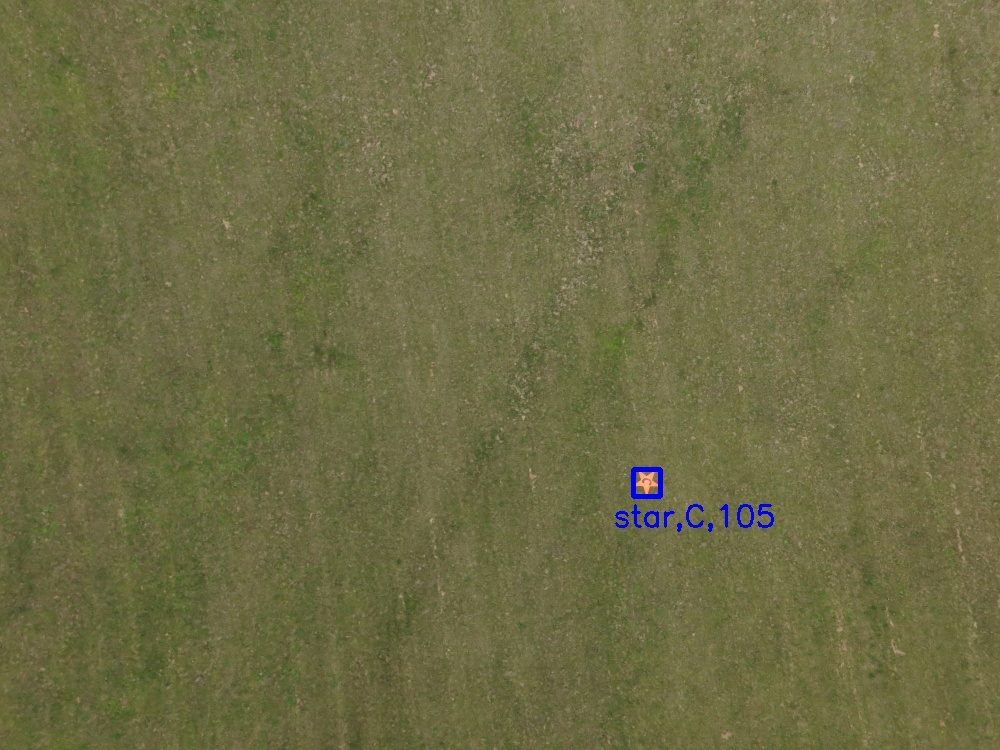
\includegraphics[width=0.8\textwidth]{true_positive_correct_letter2}
	\caption{Target classified correctly as: shape=star, char=C and angle=$105^\circ$.}
	\label{fig:true_positive2}
\end{figure}

\subsection{Low Power Computing}

The Jetson TK1,~\cref{fig:jetson}, and its predecessor, the Jetson TX1~\cite{jetsontk}, offer
both a general purpose CPU and a powerful GPU in a low power
($<10[\textrm{W}]$), small form factor plaform ($10\textrm{x}10[\textrm{cm}]$).
The GPU enables fast calculation of DL networks. Using the Jetson TK1 and the
Caffe~\cite{jia2014caffe} DL network, we are developin a low power, real-time
target detection and classification system. The later enables fast calculation
of the DL network.
\begin{figure}[h]
	\centering
	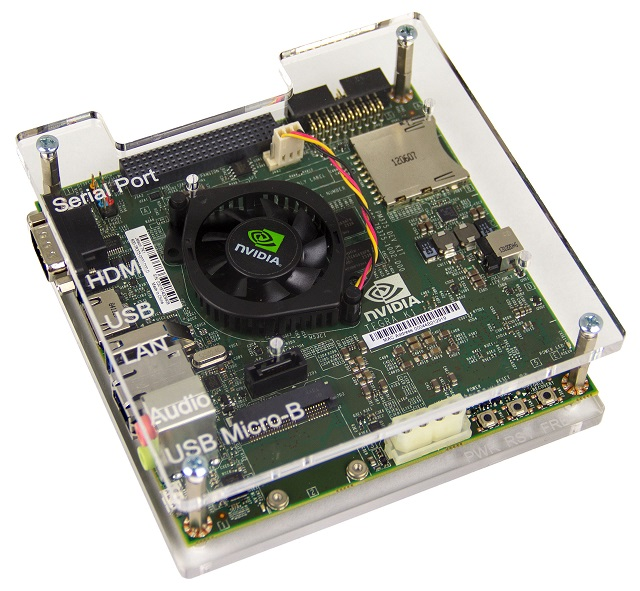
\includegraphics[width=0.8\textwidth]{jetson}
	\caption{The Jetson TK1 by NVIDIA}
	\label{fig:jetson}
\end{figure}

Initial results of running the target detection and classification algorithm on
the jetson are shown in the~\cref{tb:jetson1}. It can be seen that even at this
stage the system can handle images at tp to 4 frames per second, which should be
enough for many applications.
\begin{table}
	\centering
	\begin{tabular}{ | l | l | }
		\hline
		Stage 										& Time [ms] 	\\ \hline
		Target Detection (CPU) 						& 183      		\\ \hline
		Low Resolution Classification (GPU) 		& 7 			\\ \hline
		High Resolution Classification (GPU)		& 15 			\\ \hline
		Total 						 				& 215 			\\ \hline
	\end{tabular}
	\caption{Timing results of the Jetson TK1}
	\label{tb:jetson1}
\end{table}
As can be seen, most of the time is spent in the target detection stage.
Our goal is Real Time detection at video frame rate. Therefore we will
explore methods of performing detection using a DL network~cite{Szegedy2013}. For
example we will test merging the detection and classification stages into a
single network~\cite{long2014fully}.

\subsection{Demonstration system}

The developed algorithms will be tested on the Technion drone~\cref{fig:drone}. This
project is developed as part of the Association for Unmanned Vehicle Systems International
(AUVSI) Student Unmanned Air Systems (SUAS) Competition~\cite{AUVSI_competition}.
\begin{figure}[h]
	\centering
	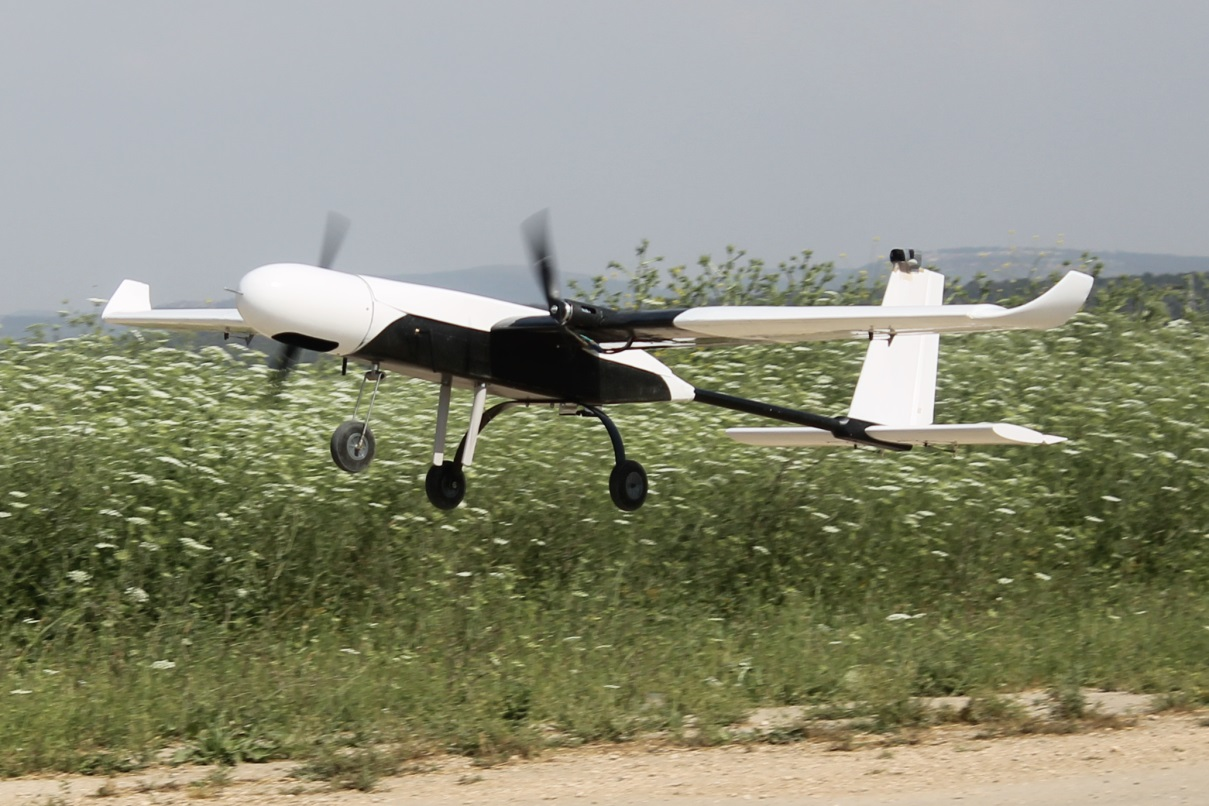
\includegraphics[width=0.8\textwidth]{drone}
	\caption{The Technion drone project.}
	\label{fig:drone}
\end{figure}
The Jetson TK will be deployed on-board the drone as part of the payload. It will process
images captured by the payload camera in Real Time. Among its tasks will be the
detection and classification of targets and humans.

\subsection{Extensions}

Other tasks for which deep learning has been proven to be very effective are
obstacle avoidance~\cite{hadsell2009learning, eigen2014depth, ross2013learning}.
This is the `Holy Grail' of UAS. 

\section{Budget Plan}

\begin{center}
	\begin{tabular}{ | l | l | l | }
		\hline
				& Item 											& Budget (NIS) 	\\ \hline
		1		& MSc Student 									& 20,000    	\\ \hline
		2		& 1 global shutter machine vision camera 		& 25,000 		\\ \hline
		3 		& 1 computer and accessories 					& 10,000 		\\ \hline
		4 		& 4 GPU Nvidia Jetson TX1	 					& 12,000 		\\ \hline
		5 		& Operating expenses (Flight tests) 			& 10,000 		\\ \hline
		6 		& Supplies and publication	 					& 8,000 		\\ \hline
		7 		& Transportation and communication				& 5,000 		\\ \hline
		8 		& Students travel 								& 20,000 		\\ \hline
		9 		& Laboratory staff (engineers \& technicians)	& 20,000 		\\ \hline
		Total 	&  							 					& 130,000 		\\ \hline
	\end{tabular}
\end{center}

\section{Mark Siberstein - Short Biography}

\bibliography{project}
\bibliographystyle{unsrt}
\end{document}



